\documentclass[12pt,prb,aps,epsf]{report}
\usepackage[utf8]{inputenc}
\usepackage{amsmath}
\usepackage{amsfonts}
\usepackage{amssymb}
\usepackage{graphicx} 
\usepackage{latexsym} 
\usepackage[toc,page]{appendix}
\usepackage{listings}
\usepackage{xcolor}
\usepackage{soul}
\usepackage[T1]{fontenc}
\usepackage{amsthm}
\usepackage{mathtools}
\usepackage{setspace}
\usepackage{array,multirow,makecell}
\usepackage{geometry}
\usepackage{textcomp}
\usepackage{float}
%\usepackage{siunitx}
\usepackage{cancel}
%\usepackage{tikz}
%\usetikzlibrary{calc, shapes, backgrounds, arrows, decorations.pathmorphing, positioning, fit, petri, tikzmark}
\usepackage{here}
\usepackage{titlesec}
%\usepackage{bm}
\usepackage{bbold}

\geometry{hmargin=2cm,vmargin=2cm}

\begin{document}
	
	\title{LP 33 Interférences à deux ondes en optique}
	\author{Naïmo Davier}
	
	\maketitle
	
	\tableofcontents
	
	\pagebreak

\section{Pré-requis}
	- Notion de chemin optique\\
	- Lentille mince\\
	- Équations de propagation d'une onde plane ou sphérique\\
	(+ Savoir ce qu'est un interféromètre)
	
\section{Introduction}
La lumière, objet de nombreuses études à longtemps fait débat quand à sa nature ondulatoire ou corpusculaire. Historiquement Young fut le premier à observer une figure d'interférences lumineuses en utilisant deux fentes placées devant une source, dispositif interférentiel portant aujourd'hui son nom. 
\paragraph{Illustrer avec fentes d'Young.}
Cette expérience met en évidence le caractère ondulatoire de la lumière car les interférences sont un phénomène intrinsèquement ondulatoire. En effet on comprend aisément que si lalumière se comportait uniquement comme un corpuscule alors on observerait seulement les projections géométriques des fentes sur l'écran.\\ 

Nous allons voir dans cette leçon comment, avec un formalisme décrivant la lumière du point de vue ondulatoire, on peut expliquer ce phénomène d'interférences. Après avoir jeté un œil sur la notion de cohérence on pourra ensuite s'intéresser aux modes opératoires permettant d'observer ce phénomène dans la pratique.
\paragraph{Remarque :} bulles de savon = coin d'air.


\section{Détecteurs (Pérez p246)}
En optique les détecteurs sont sensibles au champ électrique $\vec{E}$ porté par l'onde lumineuse. Cependant les détecteurs ont un temps caractéristique très long devant celui du champ, étant de l'ordre de $1/24s$ pour l'œil humain et de $10^{-12}s$ pour une photo-diode contre $10^{-14}s$ pour le champ porté par une onde lumineuse. Par conséquent le champ oscille trop vite pour le détecteur qui ne peut ainsi mesurer que sa valeur moyenne $\langle\vec{E}(t)\rangle_{\tau_{detecteur}} \simeq 0$ car $\tau_{detecteur} \gg \tau_{lumiere}$. On va donc s'intéresser à l'éclairement $\acute{E}$ en $Wm^{-2}$ qui est proportionnel à $\langle\vec{E}^2(t)\rangle$ ($\acute{E}= \frac{n\langle\vec{E}^2(t) \rangle}{2\mu_0c}$) car ce dernier sera donc non nul et ainsi sa mesure sera pertinente.

\section{Superposition de deux ondes monochromatiques (Pérez p282)}
\subsection{Cas de deux ondes planes monochromatiques}
On considère deux ondes lumineuses, planes, monochromatiques et de pulsation $\omega_1$ et $\omega_2$, décrites par 
\begin{eqnarray}
\underline{\vec{E}}_i(\vec{r}, t) = E_i e^{i(\vec{k}.\vec{r} - \omega_it+\phi_i)}\vec{\underline{e}}_i \hspace{2cm} i=1,2
\end{eqnarray}
où les vecteurs $\vec{\underline{e}}_i$ sont les vecteurs unitaires portant la direction polarisation et les $\phi_i$ les phases de vibrations.
\paragraph{Remarque:} On peut surligner ici le fait que l'expression réelle du champ est la partie réelle du champ complexe explicité ici, et que l'on fait le choix de se placer en complexe car la linéarité des équations de Maxwell nous le permet, et que l'exponentielle est bien utile étant la base propre de la dérivée.\\
 Si ces deux ondes se superposent au point M le champ résultant sera, par linéarité des équations de Maxwell, la somme des deux champs associés à chaque onde, on aura donc $\underline{\vec{E}} = \underline{\vec{E}}_1 + \underline{\vec{E}}_2$. Or on s'intéresse à l'éclairement, qui est proportionnel à la moyenne du carré de ce champ
\begin{eqnarray}
|\underline{\vec{E}}|^2 = |\underline{\vec{E}}_1|^2 +|\underline{\vec{E}}_2|^2 +2Re\{\underline{\vec{E}}_1^*\underline{\vec{E}}_2\},
\end{eqnarray} 
on aura donc que l'éclairement au point M est la somme des éclairements dûs aux deux sources séparément, plus un terme d'interférences :
\begin{eqnarray}
\acute{E}(M) = \acute{E}_1(M) + \acute{E}_2(M) + 2\alpha E_1E_2\, Re \langle  e^{i(\Delta\omega t+\vec{\Delta k}.\vec{r}+\Delta\phi)} \rangle \vec{\underline{e}}_1^*.\vec{\underline{e}}_2
\end{eqnarray}
où $\alpha= \frac{n}{2\mu_0c}$, $\vec{r}=\vec{OM}$, $\Delta\omega=\omega_2-\omega_1$, $\Delta k = \vec{k}_2-\vec{k}_1$ et $\Delta\phi=\phi_2-\phi_1$. On voit que l'éclairement sera uniforme et simplement la somme des deux éclairements si les deux sources responsables de l'émission de ces ondes sont incohérentes. Pour que le terme d'interférence soit non nul il faut que $\Delta\omega=0$, et donc que les deux ondes soient isochrones, et que les directions de propagation des deux ondes ne soient pas orthogonales. Pour la suite on va donc se placer dans le cas idéal $\omega_1=\omega_2$ et $Re(\vec{\underline{e}}_1^*.\vec{\underline{e}}_2)=1$.

\paragraph{Remarque :} On voit ici que l'annulation du terme d'interférence pour $\omega_1 \neq \omega_2$ correspond à "deux ondes de fréquences différentes n'interfèrent pas entre elles".

\subsection{Cas de deux OPM isochrones}

\begin{figure}[h]
	\centerline{ 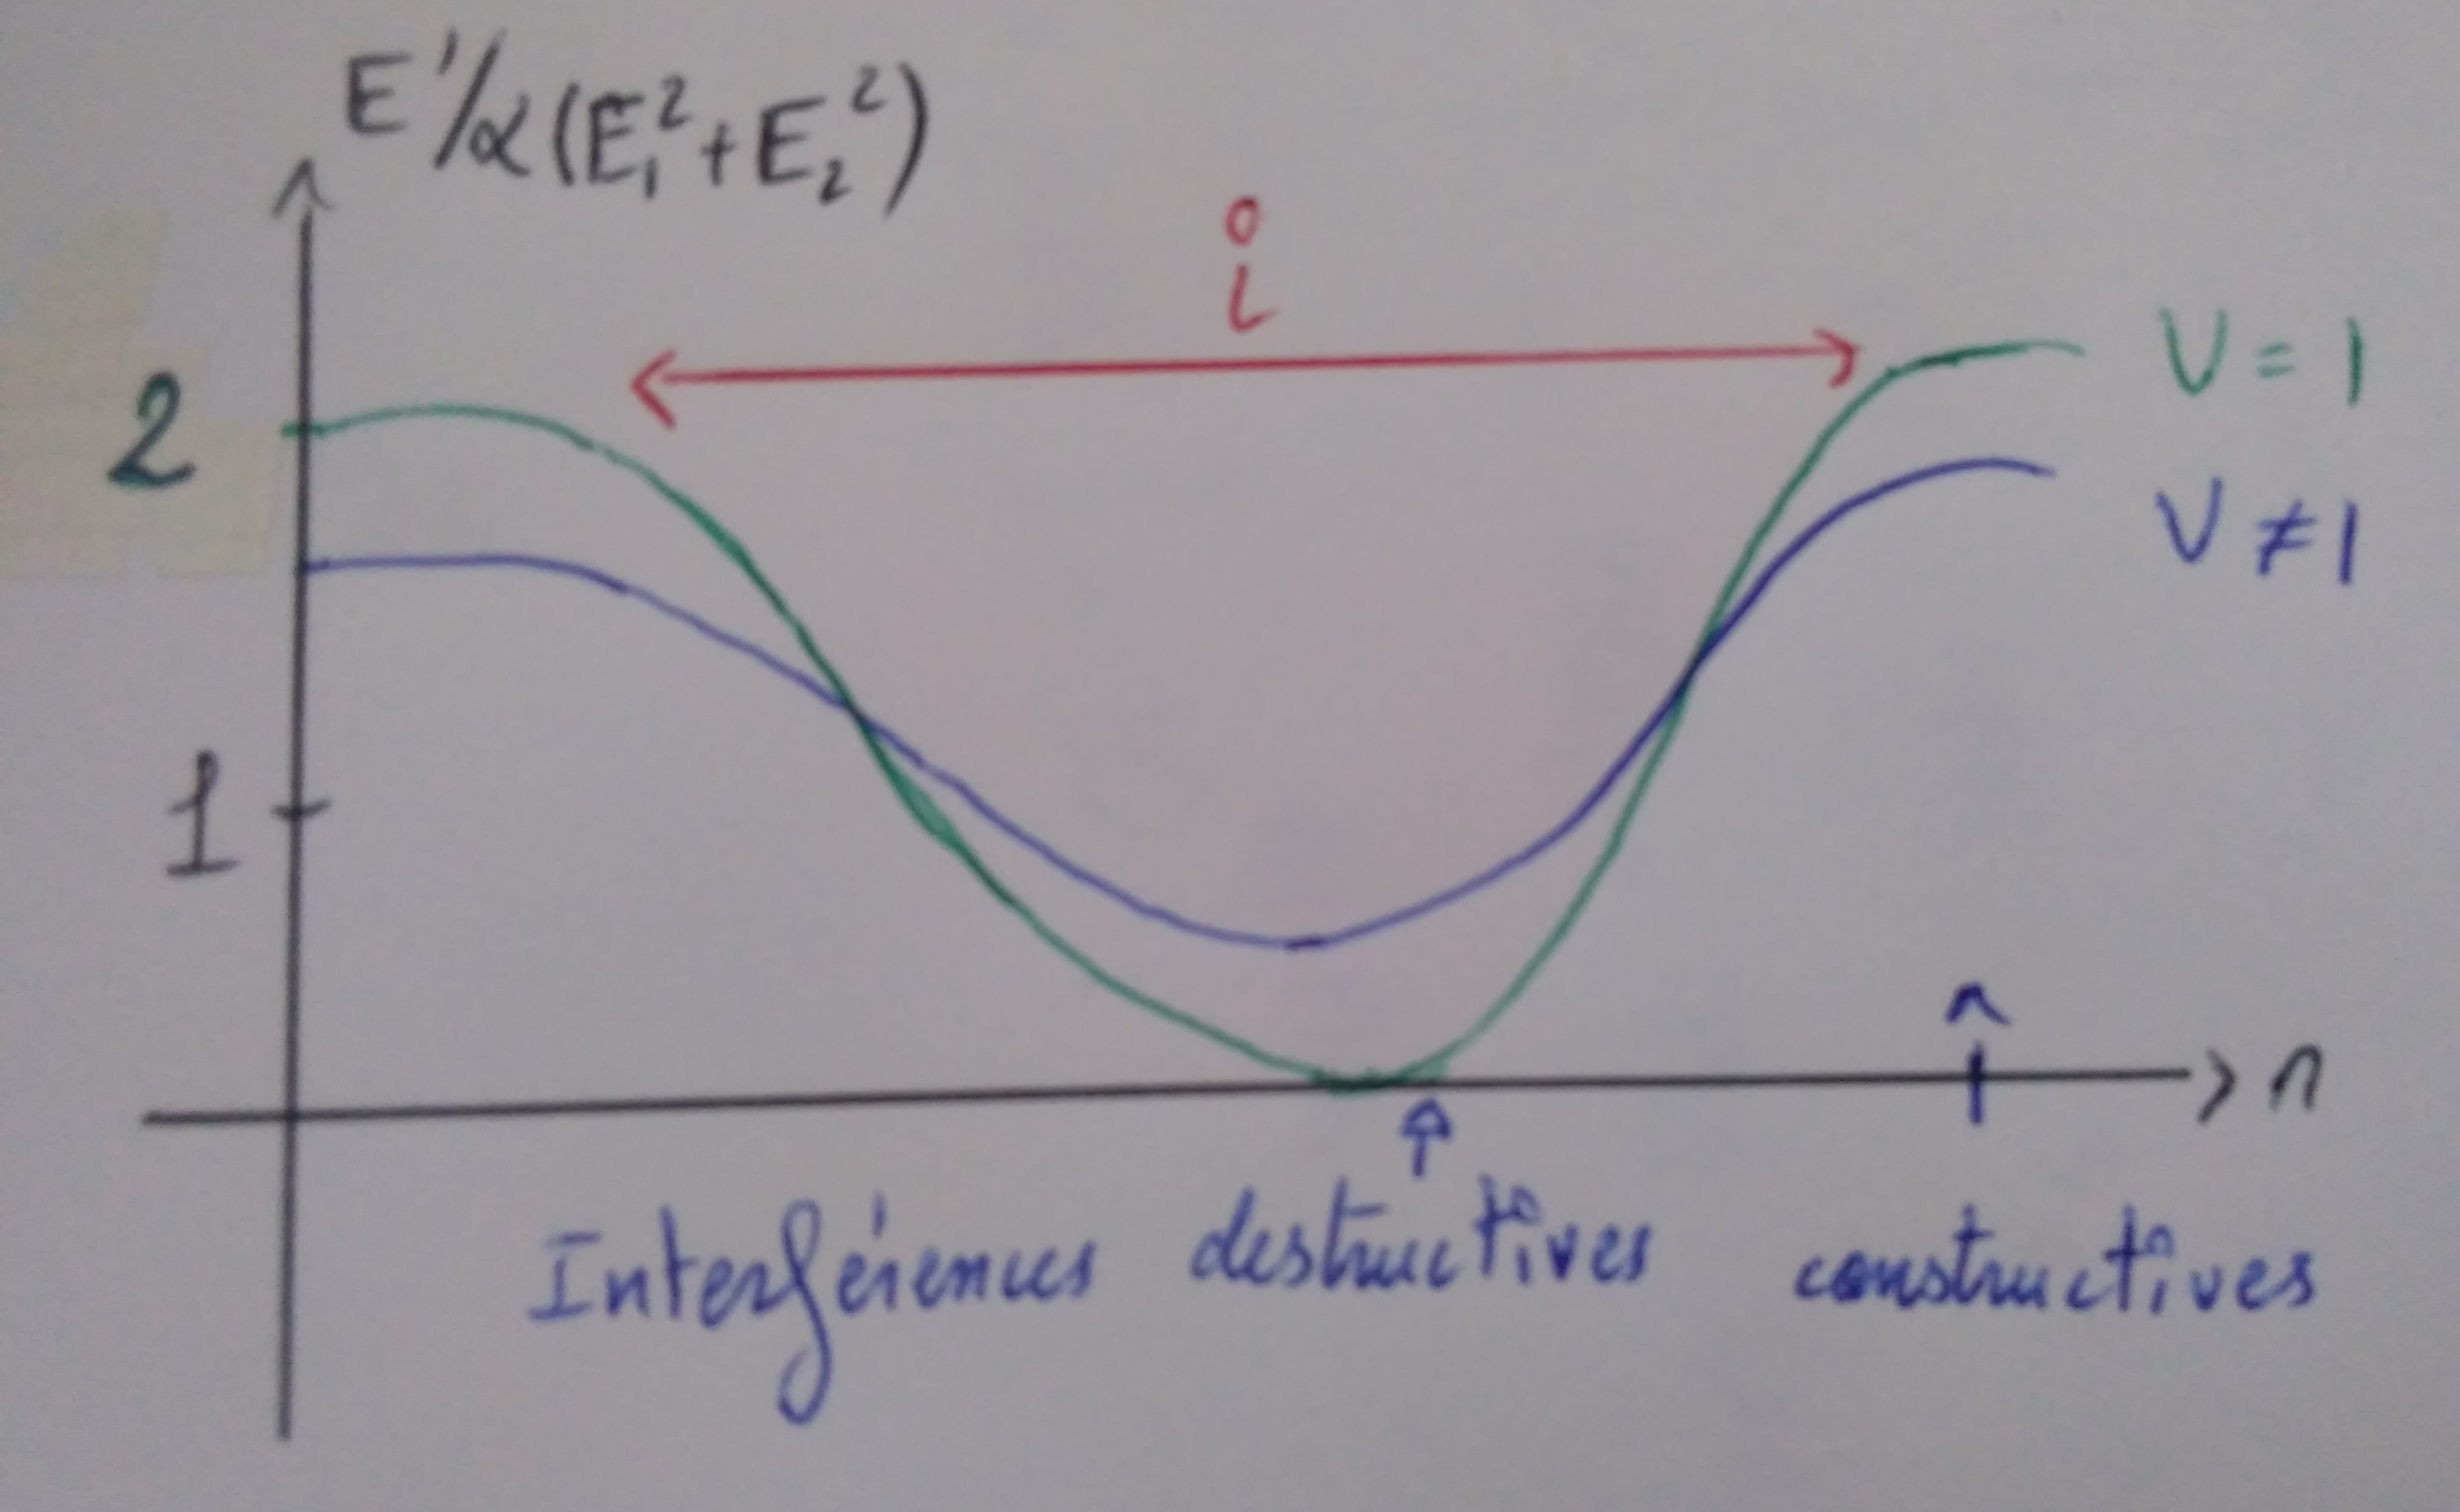
\includegraphics[width=8cm]{2OPPM}}
\end{figure}
Dans ce cas on a 
\begin{eqnarray}
\acute{E} &=& \acute{E}_1 +\acute{E}_2 + 2 \sqrt{\acute{E}_1\acute{E}_2}\,cos(\vec{\Delta k}.\vec{r}+\Delta\phi) \\
&=& (\acute{E}_1 +\acute{E}_2)\left(1+\frac{2 \sqrt{\acute{E}_1\acute{E}_2}}{\acute{E}_1 + \acute{E}_2}\,cos(\vec{\Delta k}.\vec{r}+\Delta\phi)\right)\\
&=& (\acute{E}_1 + \acute{E}_2)\left(1+V\,cos(\vec{\Delta k}.\vec{r}+\Delta\phi)\right)
\end{eqnarray}
où $V=\frac{2 \sqrt{\acute{E}_1\acute{E}_2}}{\acute{E}_1 + \acute{E}_2}$ $\in [0,1]$ est la visibilité. On peut ainsi définir l'interfrange $i$ comme étant la distance entre deux interférences constructives et donc entre deux franges brillantes.\\

\subsection{Cas de deux OS isochrones}
Cette fois ci on considère des ondes sphériques, toujours isochrones, émises pas deux sources ponctuelle $S_1$ et $S_2$. Ici la valeur du champ ne dépend plus du vecteur d'onde mais seulement de la distance à la source, on a donc
\begin{eqnarray}
\underline{\vec{E}}_S(M) = \frac{E}{SM} e^{i(kSM +\phi_i)}\vec{e}
\end{eqnarray}
où $r_i = ||\vec{S_iM}||$ est la distance entre la source $S_i$ et le point $M$ auquel on observe le champ. On va donc avoir au point $M$
\begin{eqnarray}
\acute{E}(M) = (\acute{E}_1 + \acute{E}_2)\left(1+V\,cos(k(S_2M-S_1M)+\Delta\phi)\right),
\end{eqnarray}
on remarque que 
\begin{equation}
k(S_2M-S_1M)=k_0(nS_2M-nS_1M)=k_0\{(S_2M)-(S_1M)\}=\frac{2\pi}{\lambda}\{(S_2M)-(S_1M)\}
\end{equation} 
et on on notera maintenant $\delta=(S_2M)-(S_1M)$ la différence de marche. On voit alors que l'on a 
\begin{eqnarray}
\acute{E}(M) = (\acute{E}_1 + \acute{E}_2)\left(1+V\,cos\left(\frac{2\pi}{\lambda}\delta+\Delta\phi\right)\right),
\end{eqnarray}
ainsi les surface iso-éclairement seront celles telles que la différence de marche $\delta$ soit nulle.\\

\begin{figure}[h]
	\centerline{ 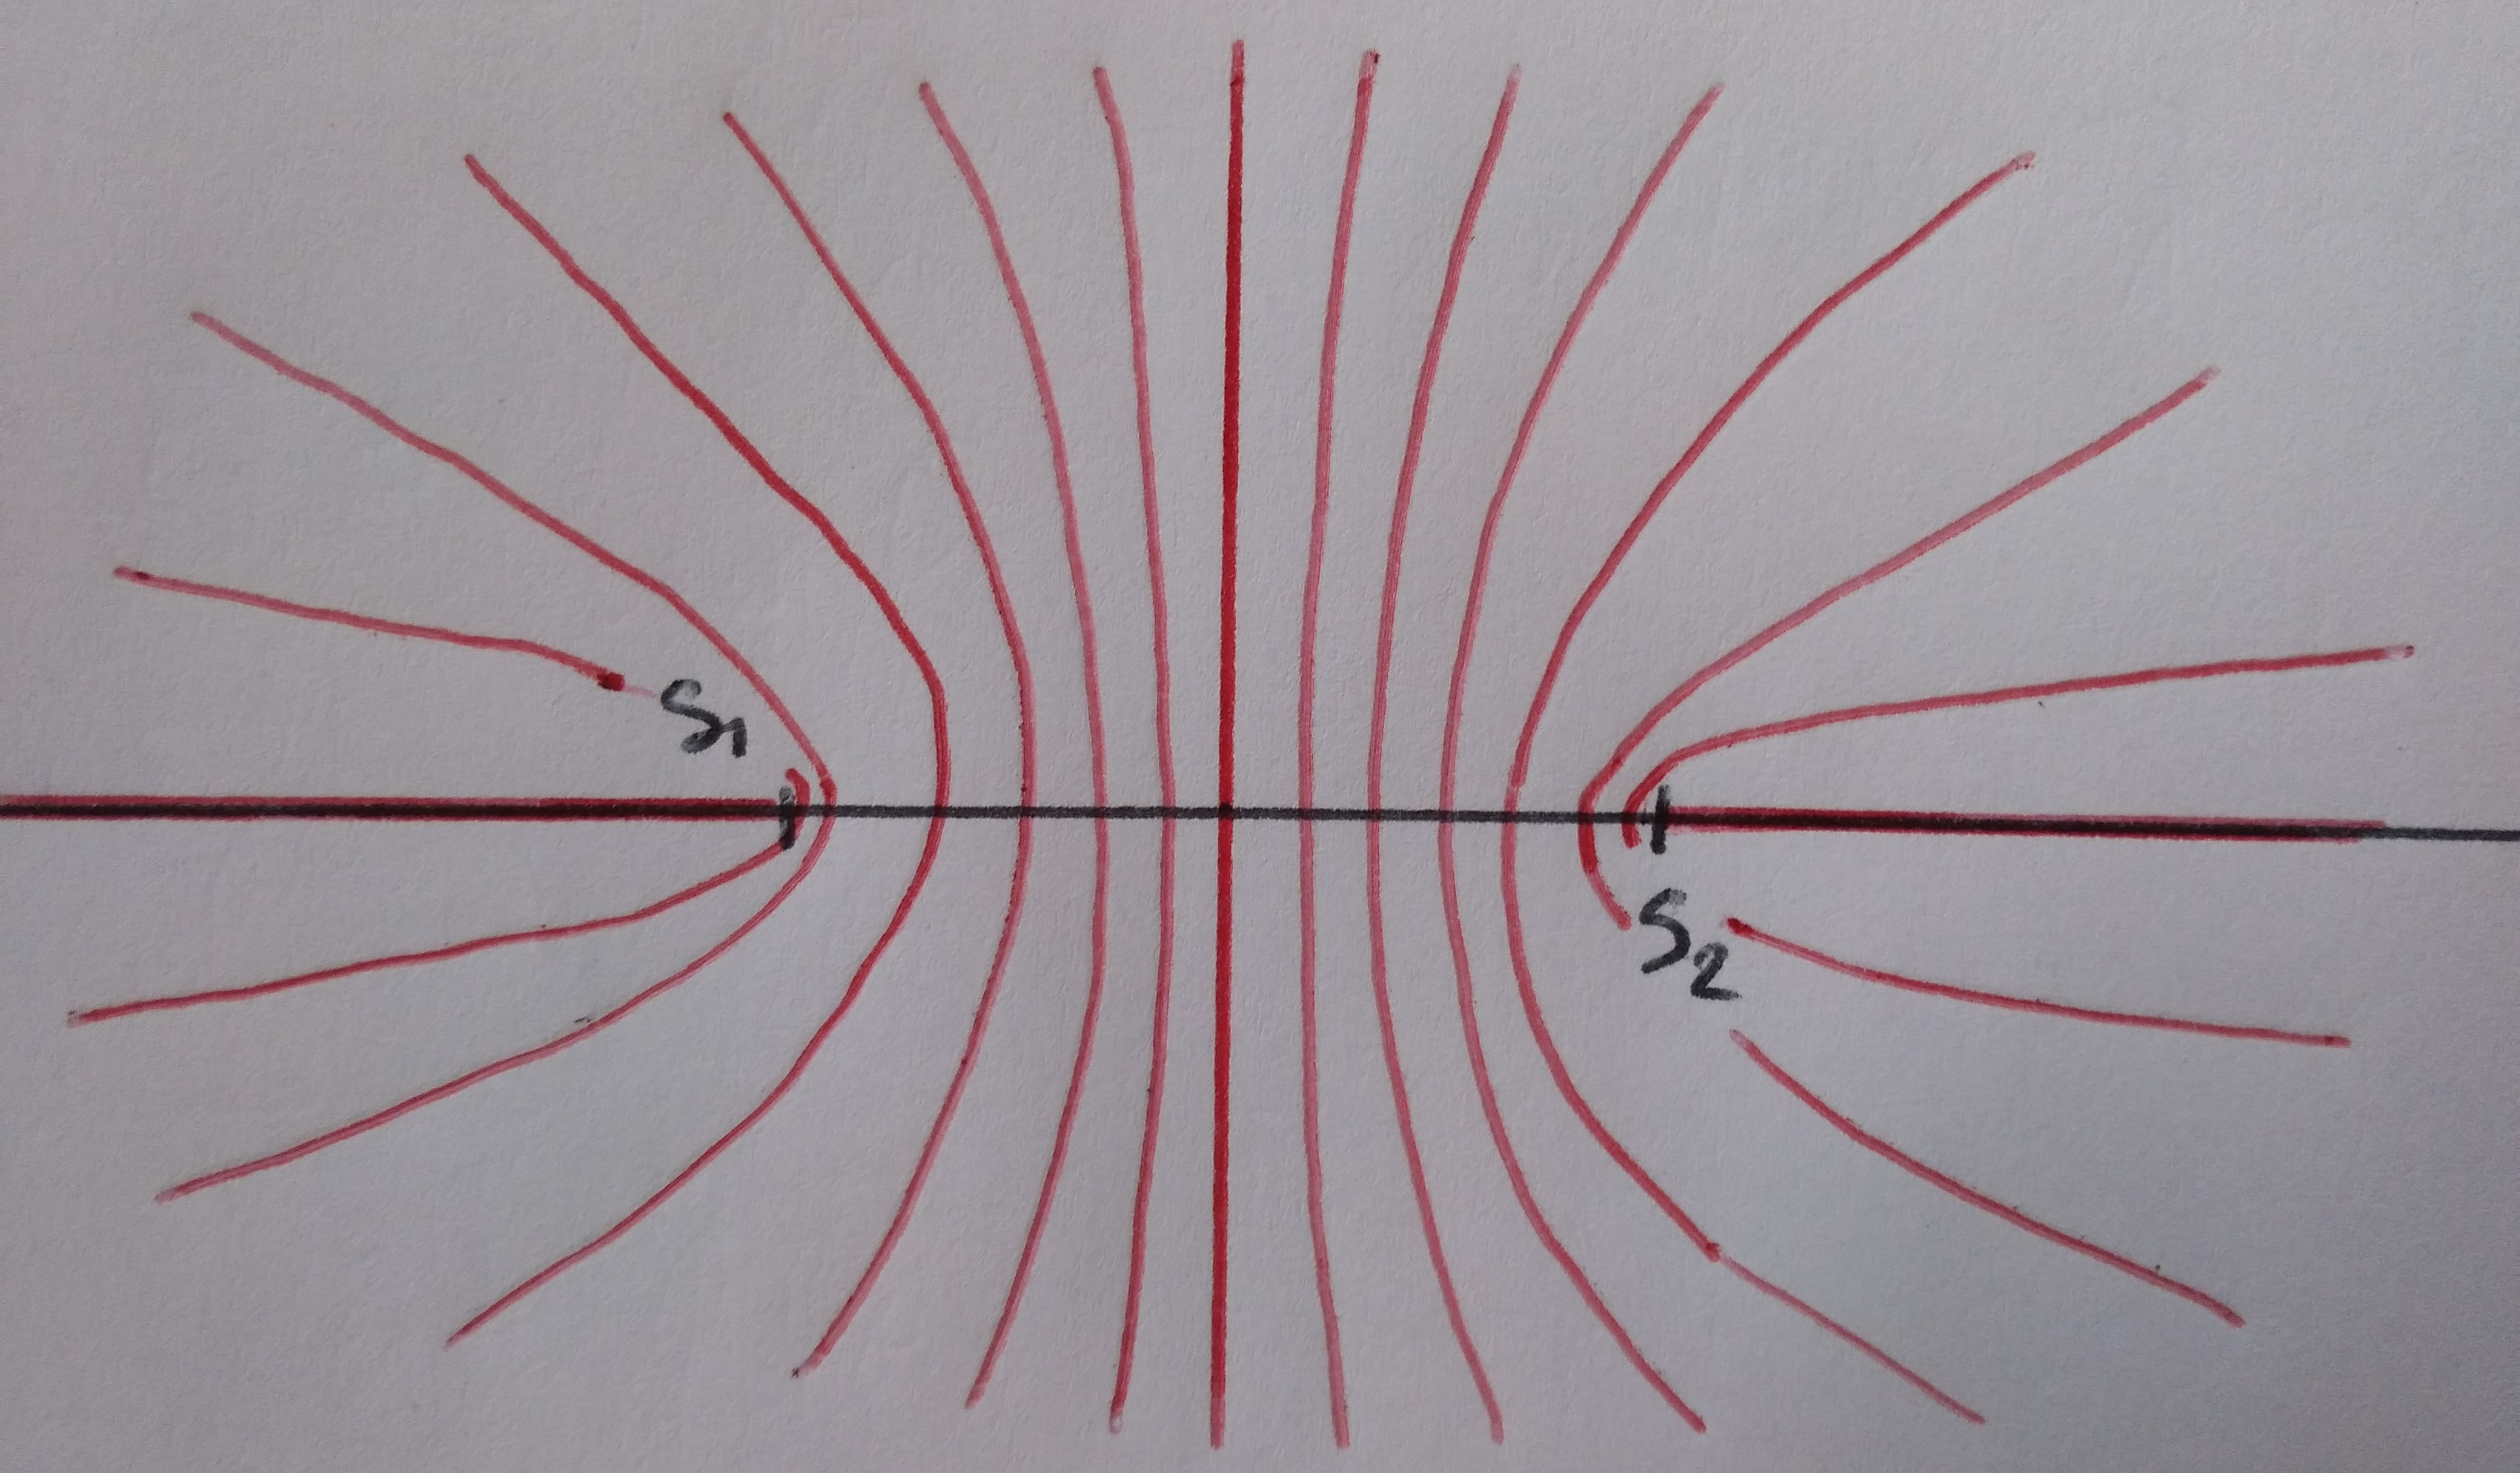
\includegraphics[width=8cm]{2OS}
				 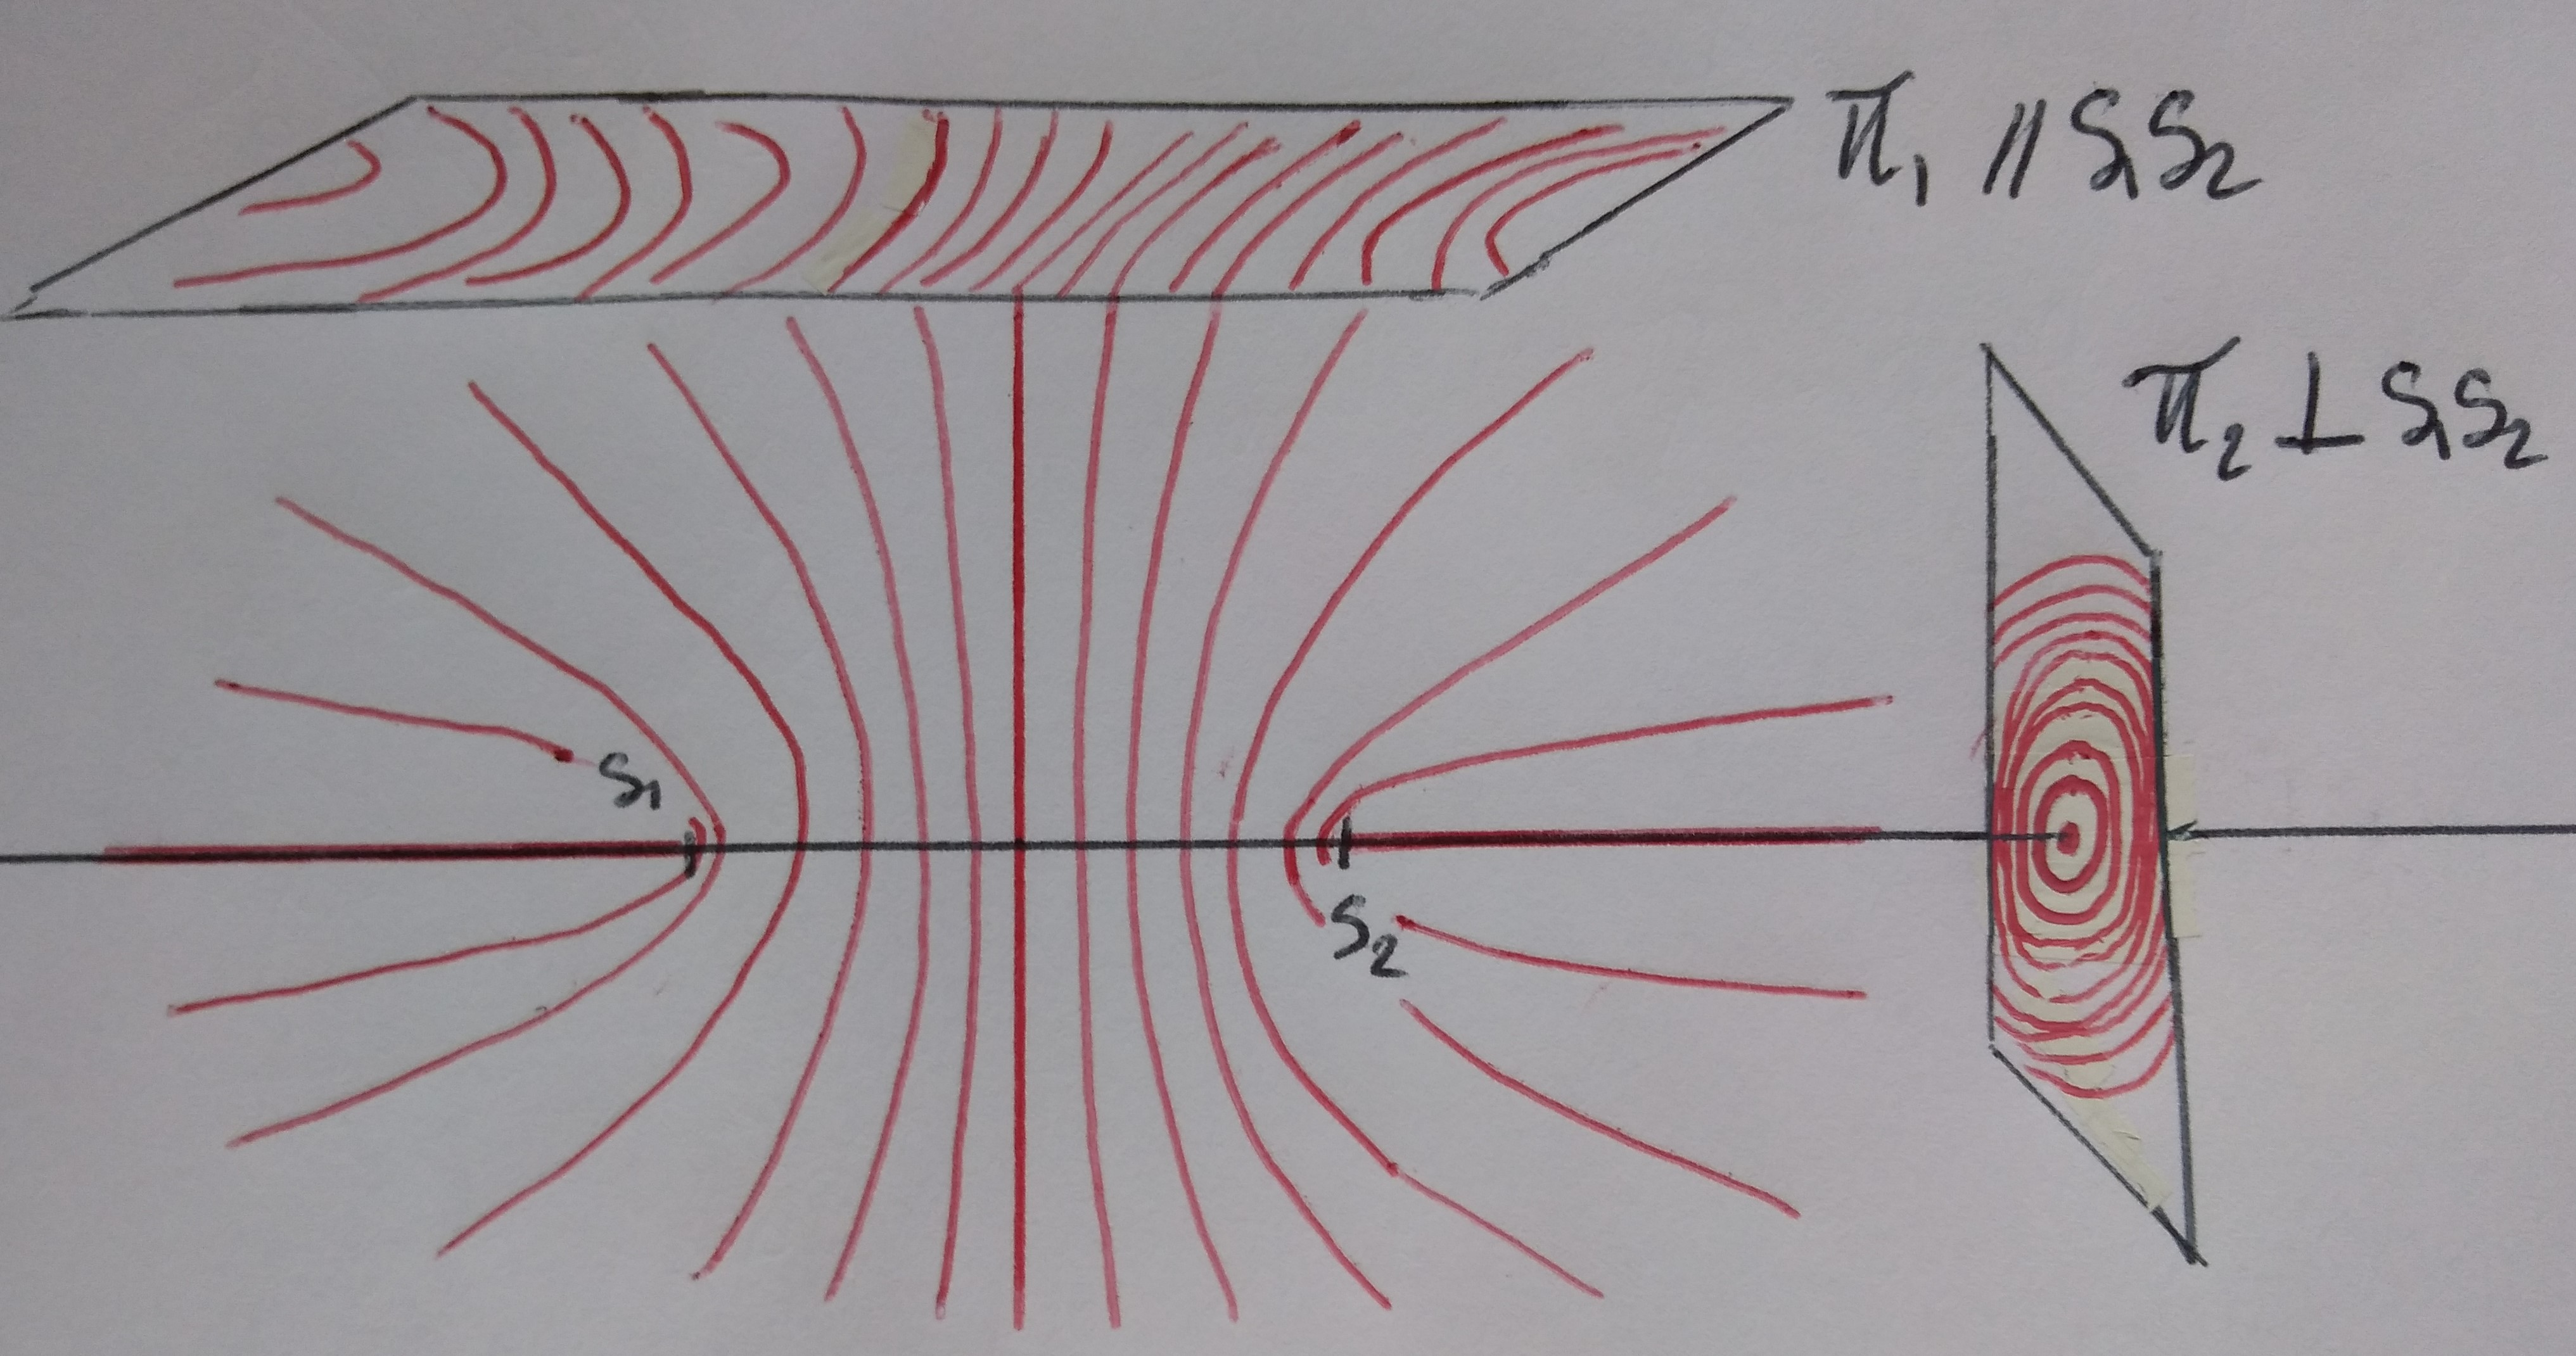
\includegraphics[width=9cm]{2OSP}}
\end{figure}

\subsubsection{Observation dans un plan parallèle à $S_1S_2$}
\begin{figure}[h]
	\centerline{ 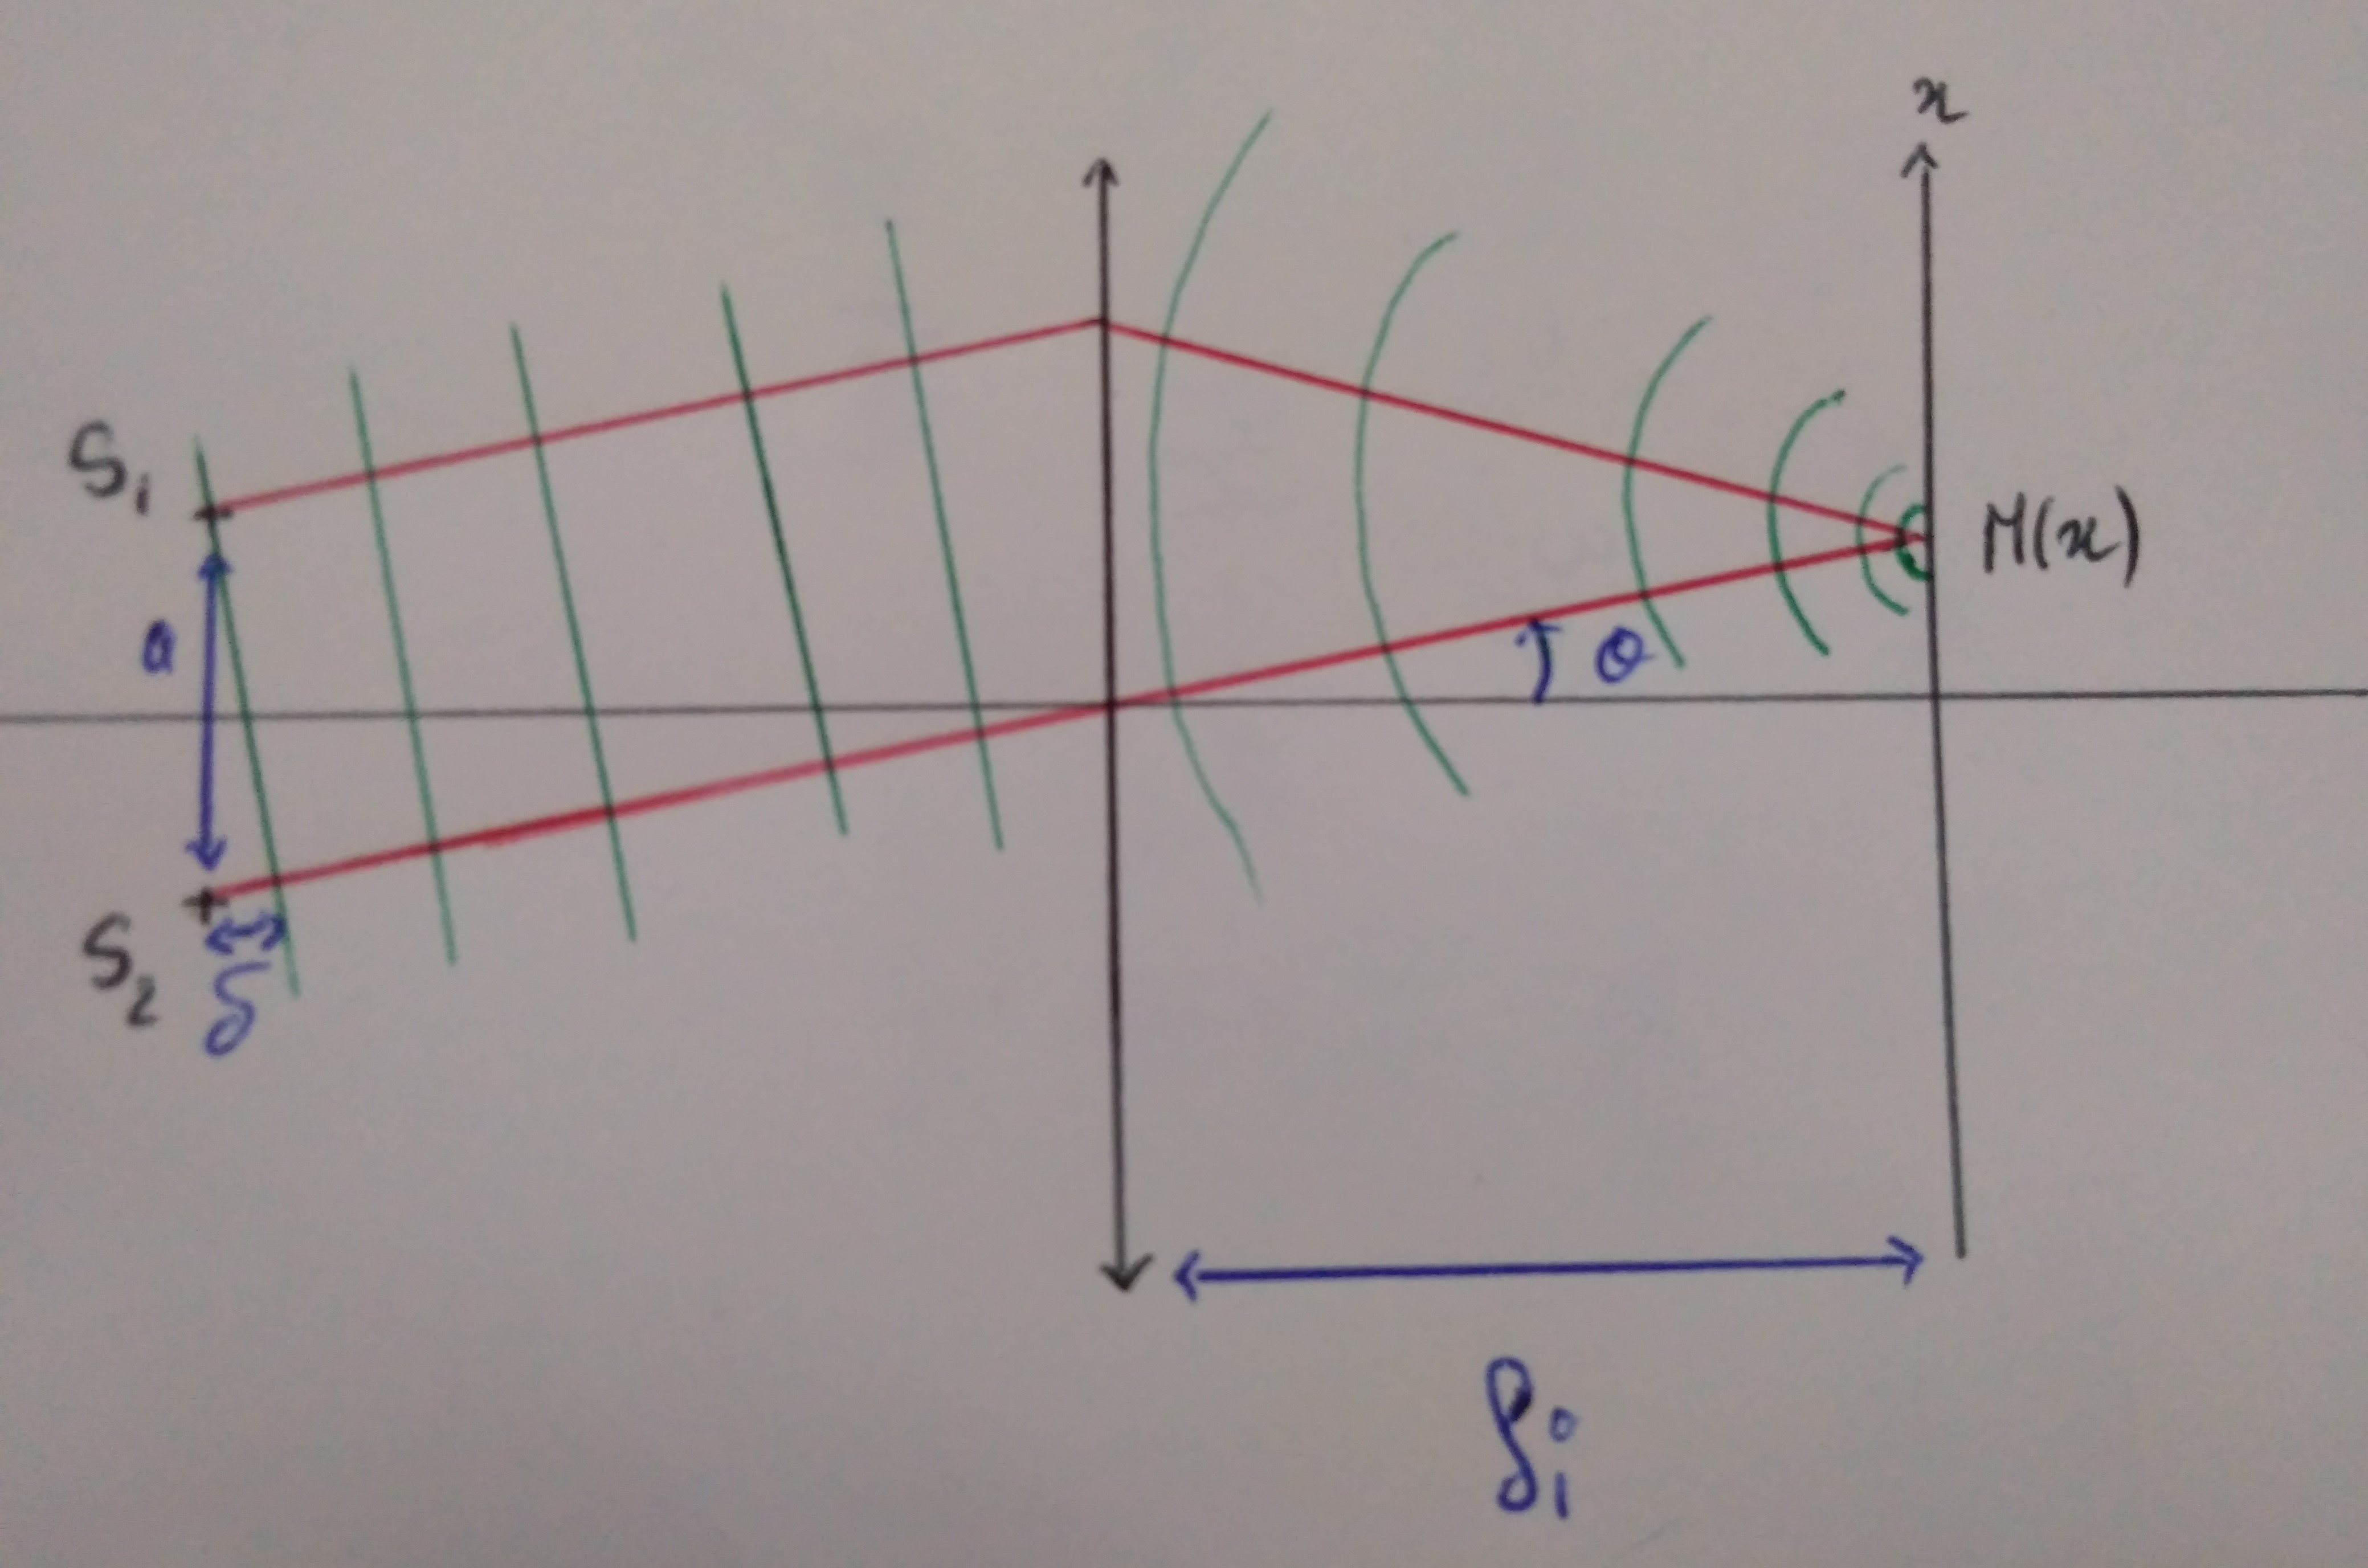
\includegraphics[width=8cm]{PparaS1S2}
				 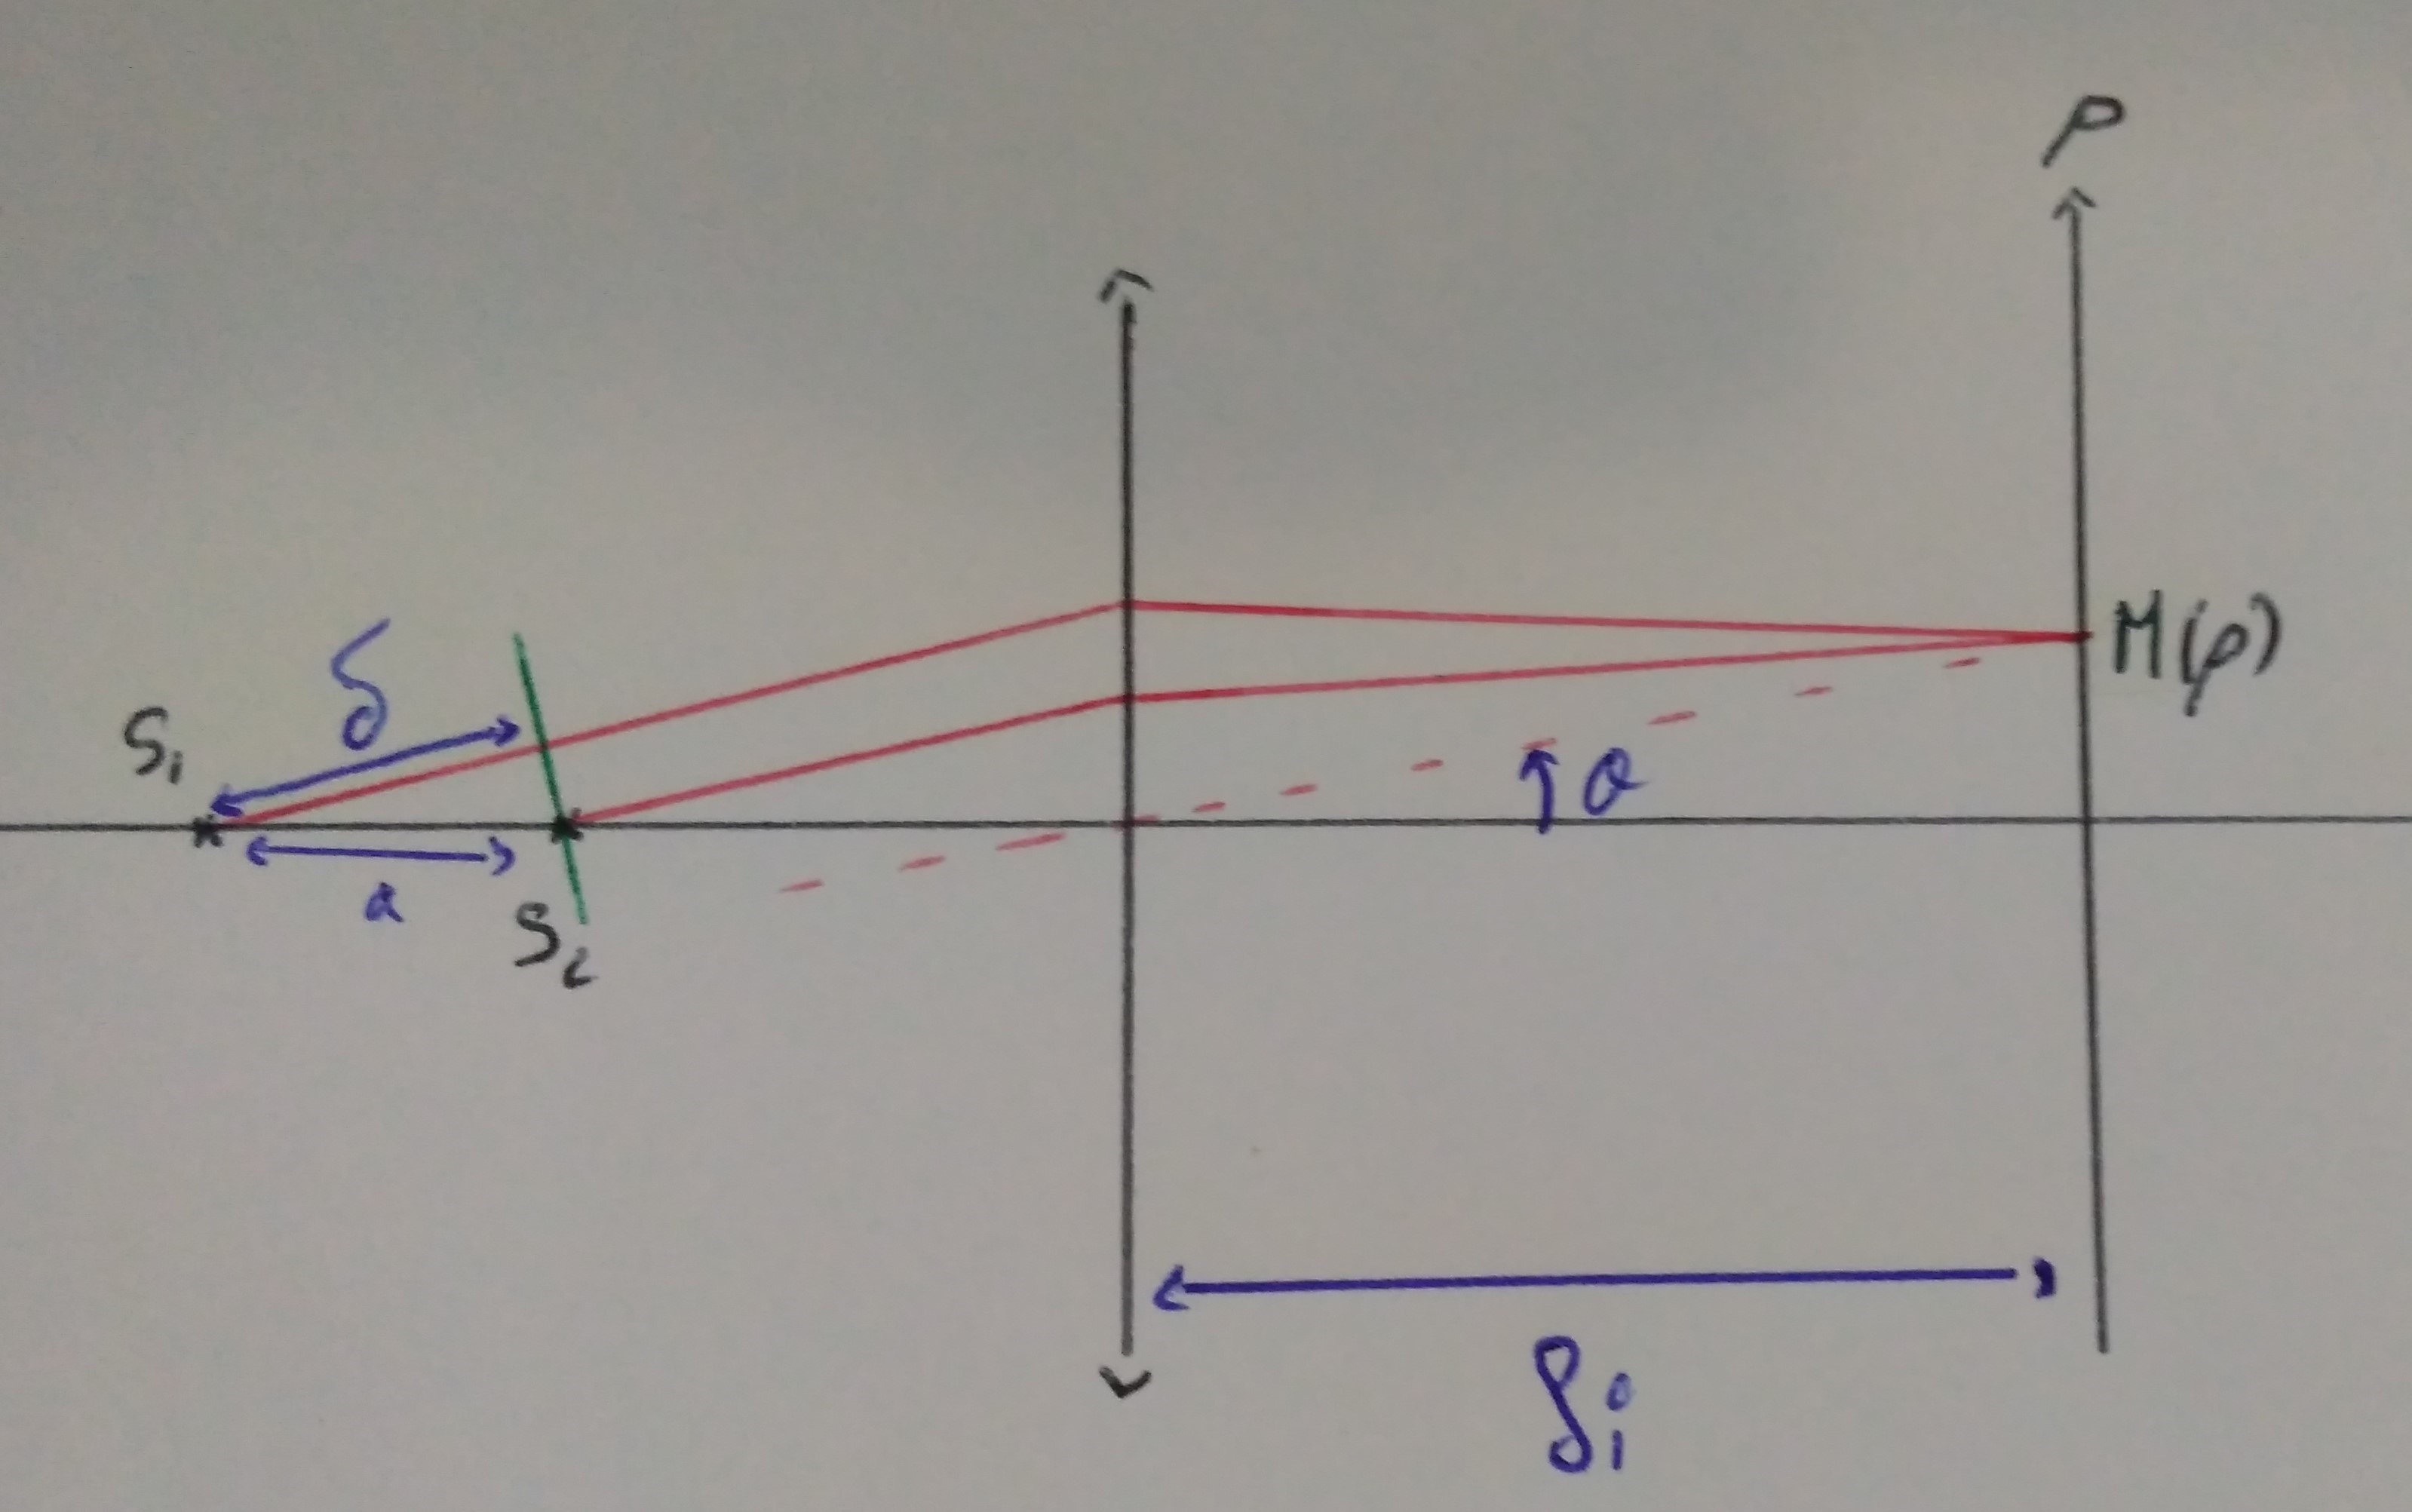
\includegraphics[width=8.5cm]{PperpS1S2}}
\end{figure}

Si la distance entre l'écran et les sources $D$ est très grande devant l'écart $a$ entre les deux sources alors on a $\delta=\frac{-ax}{f_i}$ et donc on observe des franges rectilignes $\bot$ $S_1S_2$ avec $ i=\frac{\lambda f_i}{a}$.

\subsubsection{Observation dans un plan $\bot$ $S_1S_2$}

Cette fois on a $\delta=a\,\cos(\theta) \simeq a\left(1-\frac{\theta^2}{2}\right) \simeq a \left(1-\frac{\rho^2}{2f_i^2} \right) $, on va donc observer des franges circulaires, de moins en moins intenses et de plus en plus serrées à mesure que $\rho$ augmente.\\

Rq: si le plan d'observation n'est ni $\bot$ ni $//$ $S_1S_2$ on observera ni des cercles ni des lignes mais des coniques ou des paraboles.

\section{notion de cohérence (Pérez p299)}
Dans la réalité, les sources ne sont pas parfaitement monochromatiques, et ne sont pas non plus ponctuelles, et on va voir que cela peu affecter notablement le modèle que l'on vient d'établir. 
\subsection{Cohérence temporelle}
Que la source soit un corps noir, une lampe à décharge ou un laser, elle ne sera jamais monochromatique et son intensité $I(\nu)$ sera donc généralement étalée autour d'une pulsation $\nu_0$, le plus souvent sous la forme d'une gaussienne ou d'un lorentzienne. La différence de phase liée à la différence de marche est de la forme $\Delta\Phi=k_0\delta=\frac{2\pi\nu \delta}{c}$, par conséquent, si on a une bande de pulsations de largeur $\Delta\omega$ alors toutes les ondes de pulsation $\nu \in[\nu_0-\Delta\nu/2,\nu_0+\Delta\nu/2]$ vont créer leur propre figure d'interférences. En effet les ondes de fréquences différentes n'interfèrent pas entre elles, la figure résultante sera ainsi la somme des figures d'interférence associées à chaque fréquence, et sera donc brouillée. La question est de savoir quelle largeur de bande $\Delta\nu$ est suffisamment fine pour que la figure d'interférence soit nette, et qu'ainsi le cas précédent soit une bonne approximation de la réalité. On peut, afin d'établir un ordre d'idées, considérer que $I(\nu)$ comme une distribution carrée de largeur $\Delta\nu$ centrée sur $\nu_0$, on peut de plus se donner comme critère la condition $\Delta\Phi \ll 2\pi$. Cela correspond à $\frac{2\pi\Delta\nu \delta}{c} \ll 2\pi$ soit $\delta \ll \delta_c$ où $\delta_c=\frac{c}{\Delta\nu}$ est la longueur de cohérence temporelle.\\
Rq: on peut exprimer $\delta_c$ en fonction de la longueur d'onde : $\delta_c=\frac{\lambda^2}{\Delta\lambda}$.
\paragraph{Ordres de grandeur}
	Lampe à valeur de mercure : $\Delta\lambda=10 nm$ et $\lambda_0=546nm\Rightarrow \delta_c\simeq30\,\mu m$.\\
	Laser hélium-néon : $\Delta\nu=1.4\, GHz$ et $\lambda_0=632.8\,nm\Rightarrow \delta_c\simeq20\, cm$.\\
	
\subsection{Cohérence spatiale}
La notion de cohérence spatiale est quand à elle liée à l'étendue spatiale de la source. Si on choisit de ne traiter que cet aspect en considérant le cas d'une source monochromatique, on obtient qu'un déplacement infinitésimal $\vec{\Delta S}$ du point source génère une différence de marche $\delta_S$ au point $M$ (ici fixé) que l'on peut déterminer comme étant
\begin{eqnarray}
\delta_S = \Delta[(SS_1M)-(SS_2M)] = \vec{\Delta S}(\vec{u_1}-\vec{u_2}) + \mathcal{O}(\|\Delta S\|).
\end{eqnarray}
Par conséquent si $\vec{u_1}=\vec{u_2}$ ( si la source est très éloignée de l'interféromètre par exemple, ou lames d'air, ou interféromètre à division d'amplitude), ou si $\vec{u_1}-\vec{u_2} \perp \vec{\Delta S}$ ce qui correspond au cas d'une fente source orientée perpendiculairement par rapport à la direction d'extension de la source, l'étendue de la source aura peu d'impact sur la figure d'interférence. Pour ce qui est de l'épaisseur de cette fente source, ce qui correspond à $\vec{u_1}-\vec{u_2} \mathbin{\!/\mkern-5mu/\!} \vec{\Delta S}$ on a 
\begin{eqnarray}
\Delta\Phi = \frac{2\pi}{\lambda} \Delta S \; 2 \sin\left( \frac{\alpha}{2} \right) \simeq \frac{2\pi}{\lambda} \Delta S  \alpha \simeq \frac{2\pi}{\lambda} \Delta S  \frac{a}{d_S}
\end{eqnarray}
où $\alpha =(\vec{u_1},\vec{u_2})$ et $d_S$ est la distance de la source à l'interféromètre. Si on pose à nouveau $\Delta\Phi \ll 2\pi$ comme condition de netteté on obtient que $\Delta S$ doit satisfaire $\Delta S \ll l_s$ pour que l'on observe des franges nettes, où $l_s=\frac{\lambda d_S}{a}$ est la largeur de cohérence spatiale.

\paragraph{Calcul de $\delta_S$ :}
\begin{eqnarray}
\delta = \delta(S)-\delta(S_0) = (Sp_1-SP_2)-(S_0P_1-S_0P_2) = (SP_1-S_0P_1)-(SP_2-S_0P_2)
\end{eqnarray}
or $\vec{SP_1} = \vec{SS_0} + \vec{S_0P_1}= \vec{\Delta S} + \vec{S_0P_1}$, d'où
\begin{eqnarray}
\|SP_1\|^2&=&\|\vec{\Delta S}\|^2+\|S_0P_1\|^2+2\vec{\Delta S}.\vec{S_0P_1}\\
&=& \|SP_1\|^2\left(1+\frac{2\vec{\Delta S}.\vec{S_0P_1}}{\|S_0P_1\|^2}+\frac{\|\vec{\Delta S}\|^2}{\|S_0P_1\|^2}\right)\\
\Rightarrow SP_1 &\simeq& \left(1+\frac{\vec{\Delta S}.\vec{S_0P_1}}{\|S_0P_1\|^2}+\frac{\|\vec{\Delta S}\|^2}{2\|S_0P_1\|^2}\right)\\
SP_1-S_0P_1 &=& \vec{\Delta S}.\vec{u_1} +  \frac{\|\vec{\Delta S}\|^2}{2S_0P_1}
\end{eqnarray}
Finalement on a 
\begin{eqnarray}
\delta = \vec{\Delta S}(\vec{u_1}-\vec{u_2}) + \frac{\|\vec{\Delta S}\|}{2}\left(\frac{1}{S_0P_1}-\frac{1}{S_0P_2}\right) = \vec{\Delta S}(\vec{u_1}-\vec{u_2}) + \mathcal{O}(\|\Delta S\|).
\end{eqnarray}

\subsection{Application à la mesure d'un doublet atomique (Pérez p304)} 
Considérons ici le cas d'un atome émettant à deux fréquences très proches, centrées en $\nu_0$ et distantes de $\Delta\nu$.On va ici voir comment mesurer cet écart $\Delta\nu$ en utilisant un interféromètre à division d'amplitude. En effet chacune des deux raies va produire sa propre figure d'interférences, car deux longueur d'ondes différentes n'interagissent pas entre elles, par conséquent l'éclairement au niveau d'un point $M$ de notre écran va être égal à la somme des éclairements liés à chacune des deux raies. En considérant que les deux raies sont aussi intenses on obtient (avec $V=1$ c.a.d un interféromètre bien réglé) :
\begin{eqnarray}
\acute{E}(M) &=& \acute{E}_0\left(2+\cos\left(2\pi\nu_1\tau \right) + \cos\left(2\pi\nu_2\tau\right)\,\right)\\
&=& 2\acute{E}_0 \left(1+\cos(\pi(\nu_1-\nu_2)\tau)\cos(\pi(\nu_1+\nu_2)\tau)\,\right)\\
&=& 2\acute{E}_0 \left(1+\cos(\pi\Delta\nu\tau)\cos(2\pi\nu_0\tau)\,\right),
\end{eqnarray}
où $\tau=\frac{\delta}{c}$. On remarque ici qu'on retrouve un éclairement similaire au cas de l'interférence de deux ondes monochromatique sauf que cette fois la visibilité $V$ est remplacée par une modulatrice $\gamma(\tau)=cos(\pi\Delta\nu\tau)=cos(\pi\frac{\Delta\lambda}{\lambda_0^2}\delta)$. On peut de plus calculer quelle est la différence de marche $\delta_c$ entre deux annulations de $\gamma(\tau)$,
\begin{eqnarray}
\delta_c = \frac{c}{\Delta\nu} = \frac{\lambda_0^2}{\Delta\lambda}.
\end{eqnarray}
Par conséquent si on est capable de mesurer $\delta_c$ avec un interféromètre en comptant le nombre de franges brillantes entre deux pertes de contraste, on sera alors capable de déterminer $\Delta\lambda$ connaissant $\lambda_0$ la longueur d'onde du doublet mesurable avec un réseau par exemple. En effet si on compte $n$ franges entre deux anulations du contraste on aura alors 
\begin{eqnarray}
\delta_c = \frac{c}{\Delta\nu} = n\frac{c}{\nu_0} \hspace{0.3cm}\Rightarrow\hspace{0.3cm} \Delta\nu = \frac{\nu_0}{n}
\end{eqnarray}
\begin{figure}[h]
	\centerline{ 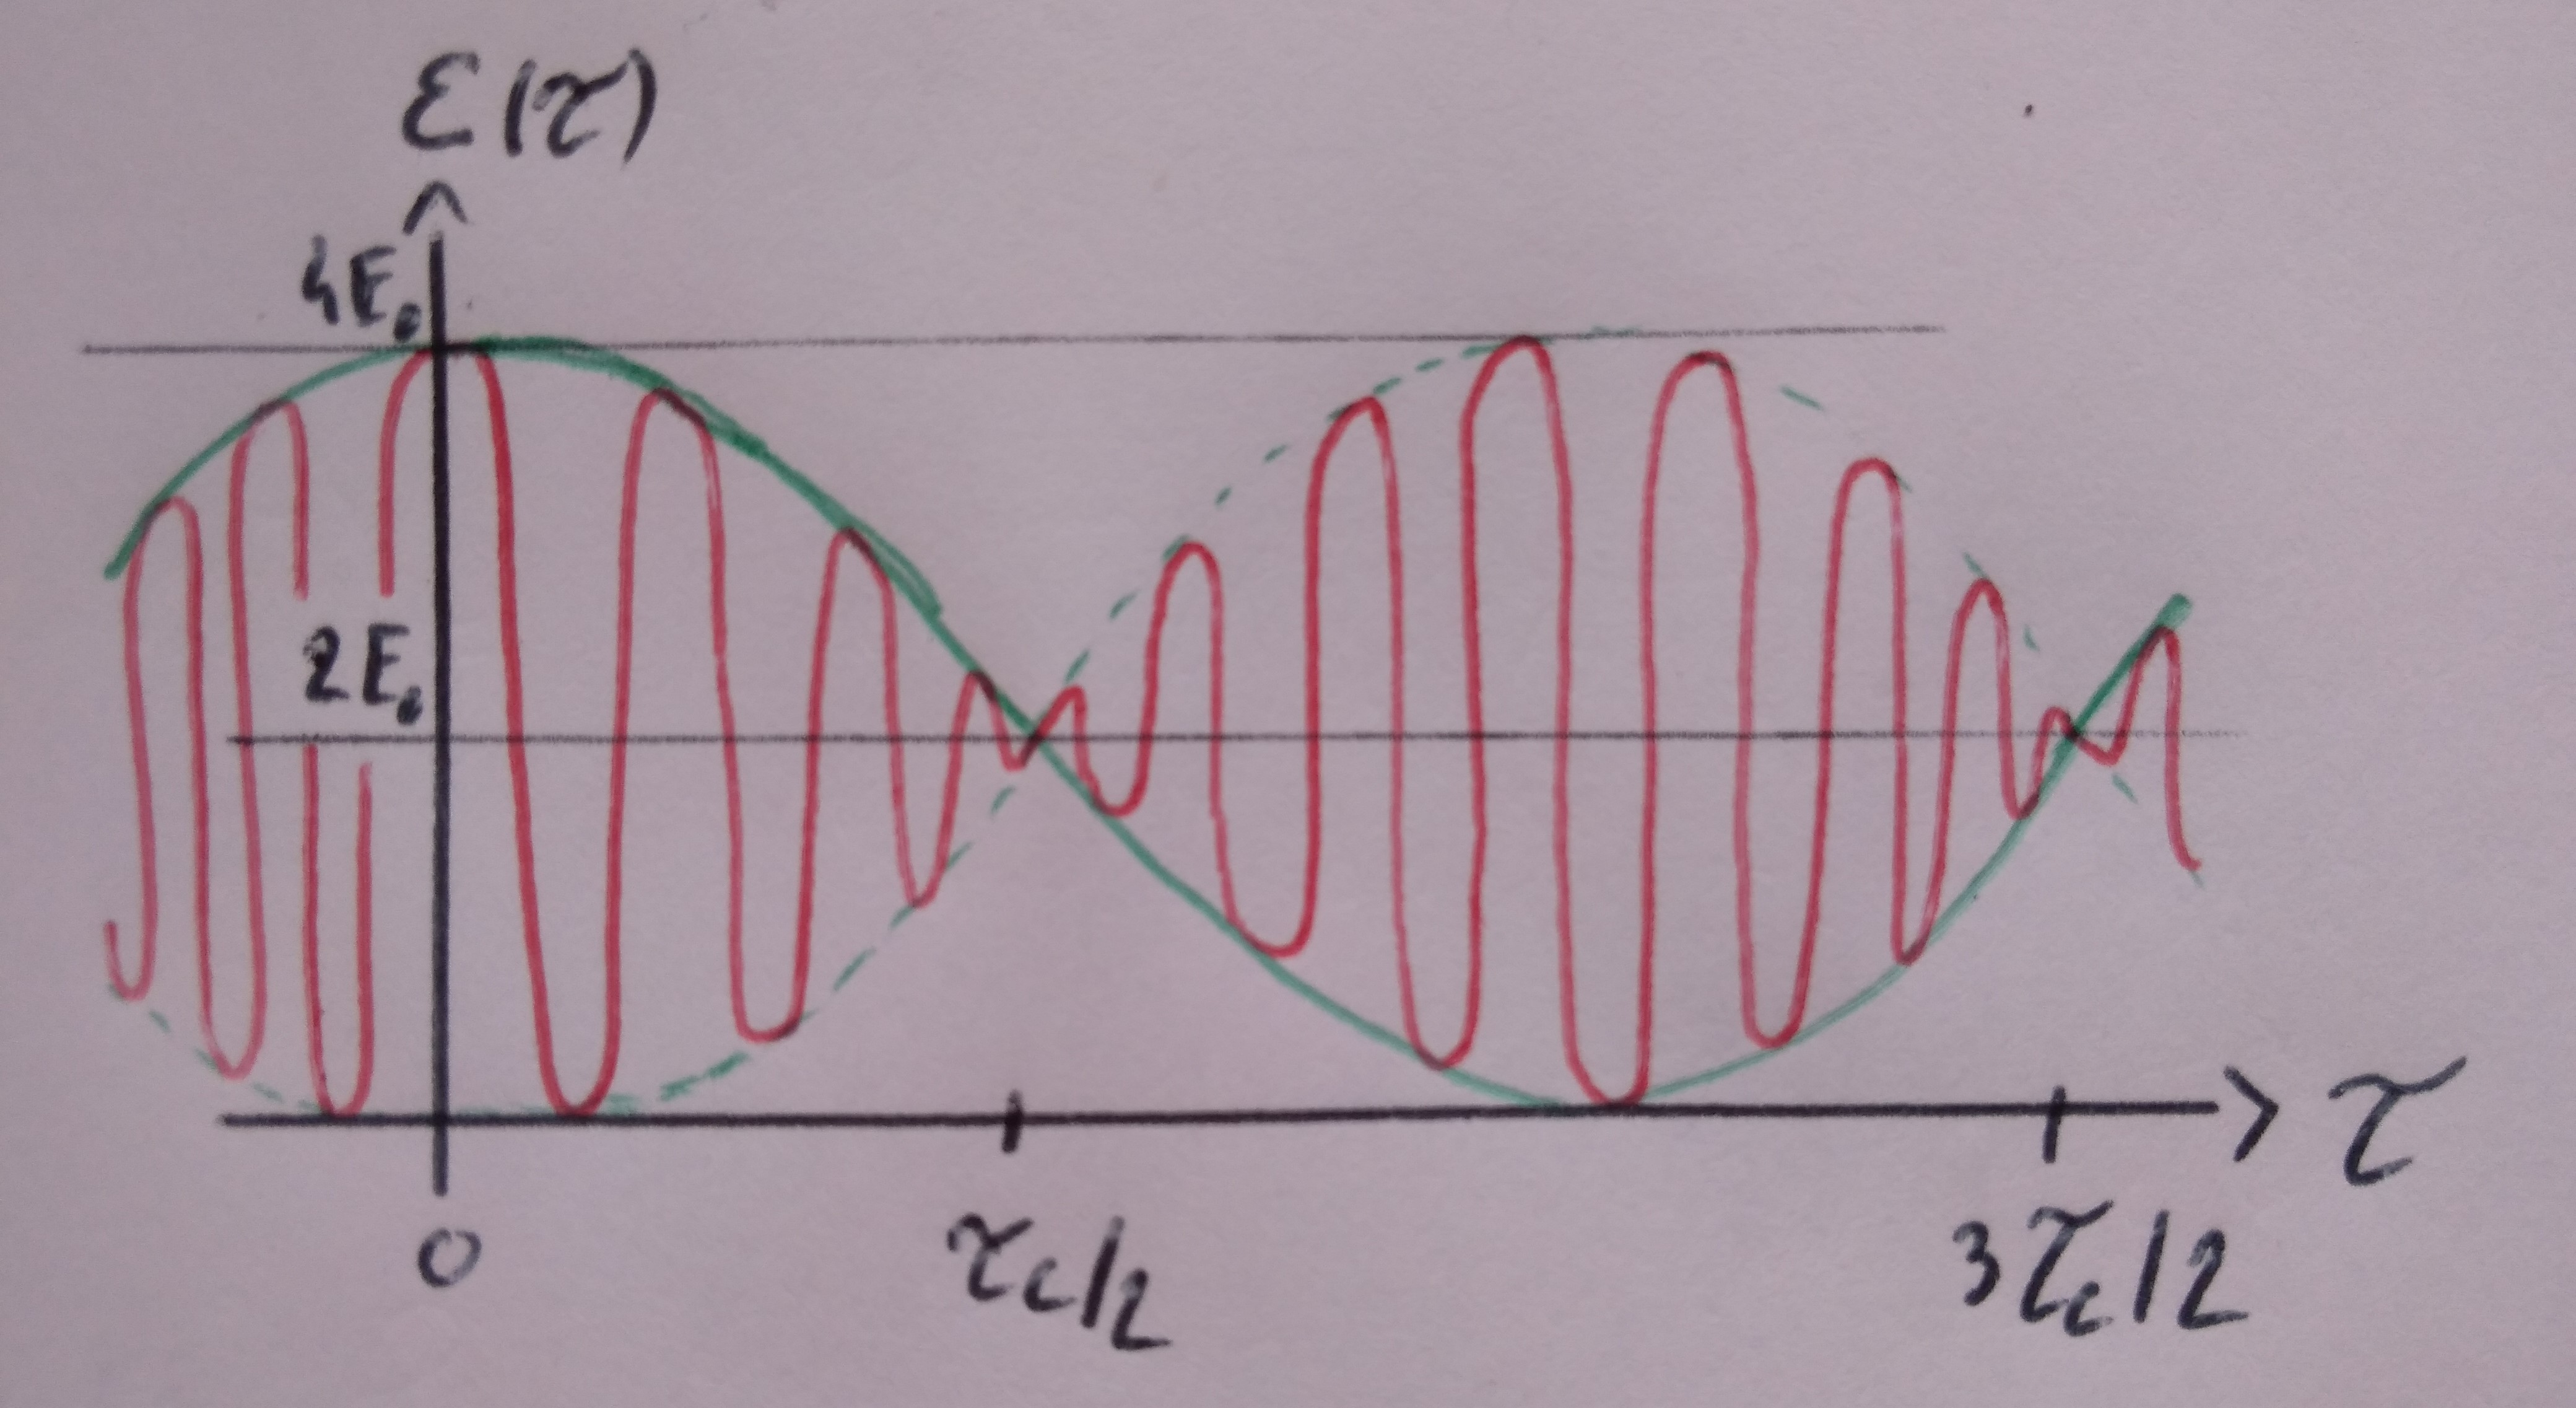
\includegraphics[width=12cm]{doublet}}
\end{figure}

\section{conclusion}
On a pu voir que le formalisme de Maxwell décrivant la lumière comme une onde permettait d'expliquer le phénomène initialement observé par Young, montrant que la lumière se comportait bel et bien comme une onde. Cependant ce phénomène est plus vaste et bien plus riche que ça, en effet il n'intervient pas seulement pour la lumière mais pour toute onde. C'est donc en utilisant les interférences que l'on a pu illustrer et étayer le paradoxe onde-corpuscule de la matière en montrant que l'on pouvait faire interférer des particules élémentaires (telles que des $e^-$ ou des $p^+$) mais aussi des molécules et même de très grosse molécules récemment. Les interférences sont donc un phénomène fondamental nous permettant d'illustrer un concept souvent abstrait.


\section{Sup: Systèmes interférentiels ou comment observer des interférences}
On a vu que à cause des problèmes de cohérence temporelle et spatiale il était impossible d'observer des figures d'interférences à l'œil si on utilise deux sources différentes, qui sont donc incohérentes. Il nous faut donc trouver le moyen de faire interagir des sources qui soient parfaitement cohérentes... et pour cela on va créer deux sources secondaires en utilisant une unique source primaire, en grâce à un interféromètre. Il existe deux grandes familles qui sont les interféromètres à division d'amplitude et division du front d'onde.\\
\begin{figure}[h]
	\centerline{ \includegraphics[width=8cm]{divfD}
		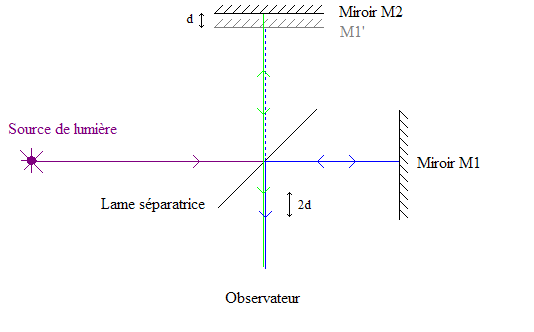
\includegraphics[width=9cm]{michelson}}
\end{figure}
\paragraph{A division du front d'onde}On utilise ici des miroirs, des fentes, des lentilles, prismes...ect pour créer deux images (au moins) d'une même source et on observe ensuite les interférences générées par les ondes provenant de ces images qui constituent des sources secondaires.

\paragraph{A division d'amplitude}L'idée de ce type d'interféromètre est de diviser un faisceau incident en utilisant une lame séparatrice et de les recombiner au bout (au moyens là encore d'une lame séparatrice) pour faire interférer ces deux faisceaux qui auront acquis un déphasage dû aux lames ajouté à celui dû à une éventuelle différence de marche.

\section{Questions}
comment on doit comprendre le $\tau = \delta /C$ ?\\
qu'est ce que l'intensité spectrale ?\\
unité de l'intensité ?\\
tout plein de détail sur les angles solides : intensité =/= éclairement \\
comment on a mesurer le doublet du sodium la premiere fois ? 

\section{Remarques} 
schémas ! \\
voca : interference =/= franges brillantes\\
intensité en watt/sterad\\
eclairement en watt/m2\\
le plan de bataille est bien mené, voire à marche forcée\\
"après ceci, on fait cela" : manque d'enchainement logique\\
problème d'homogénéité impardonnable\\
prendre le temps d'interpréter les équations\\
aucun calcul de réaliser\\
rythme de la leçon adapté au format en 40min\\
Détails techniques : \\
"mon, ma ..."\\
"l'idée c'est que "\\
"le point là c'est"\\
"si on regarde cela"\\
prendre la leçon à son compte\\
gaffe aux jugements de valeurs !!\\
gaffe aux anachronismes scientifiques\\
"on veut que" -> "ainsi"\\
"si je puis dire" -> dangereux car non précis\\
la spécificité de l'optique est que les détecteurs sont quadratiques\\
plan par une hyperboloïde c'est une patate\\
en bref travailler la rigueur du langage selon Mr.Mathevet\\
La manip à revoir\\
polarisation = vecteur complexe\\
$\omega t +\vec{k}.\vec{r} \Rightarrow$ l'onde se propage selon $-\vec{k}$

\end{document}